\subsection{Inference}
\label{inference}

As shown in Figure \ref{figure:inference}, he inference phase consists of two main steps: template matching to obtain the 3D coordinates of characteristic points and 3D dimensions for the objective vehicle and 2D-3D matching to recover the 3D vehicle location and rotation.

\begin{figure}[h]		
	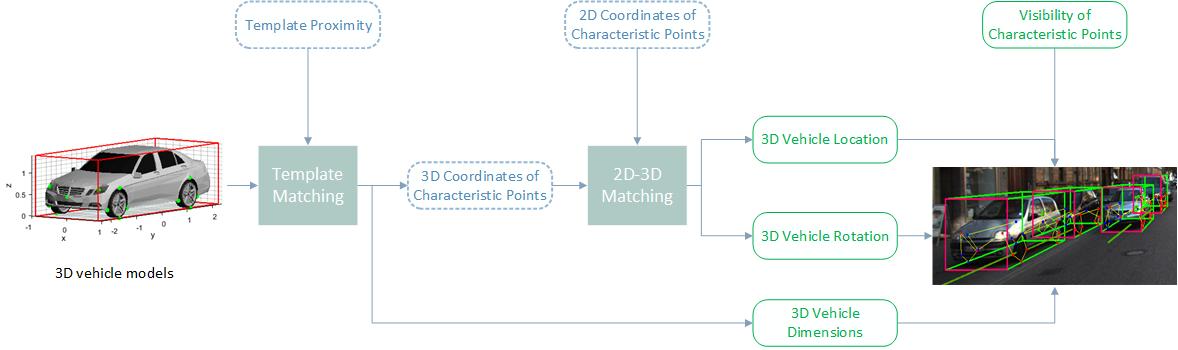
\includegraphics[width=1\textwidth]{inference_0522.png}
	\caption{The Architecture of our Approach}
	\centering
	\label{figure:inference}
\end{figure}

\subsubsection{Template Matching}

Template matching is based on the 3D template dataset and the learned template proximity for the objective vehicle in image. As defined in section \ref{template}, template proximity vector, ${T} = \{{(r_h,r_w,r_l)}_k\}_{k \in \{1,.., K\}}$, measures the dimension similarity between the target vehicle and 3D vehicle models. The best matching model is the one whose dimensions $(h, w, l)$ has the least distance to the target vehicle's dimension $(\bar{h}, \bar{w}, \bar{l})$, \ie the corresponding scaling ratios, $(r_h,r_w,r_l)$, is closest to $(1, 1, 1)$. 

Let's denote the best matching template for the target vehicle $m$ as $t_j$ and the dimension ratio between the target vehicle and the best matching model as $r_j = (r_h,r_w,r_l)$. Then its corresponding 3D sketch is $S_j^{3d}  = (p_1, p_2, ... p_{20})$. To get the target vehicle's dimension $D_m$, we apply the scaling ratios, $(r_h,r_w,r_l)$, to $t_i$ as
\begin{equation}
	D_m = t_j \cdot r_j =  (h_j, w_j, l_j) \cdot (r_h,r_w,r_l) = (h^m, w^m, l^m)
\end{equation}

In the same way, we can get the 3D coordinates of the interest points of the objective vehicle,$C_m^{3d}$, as
\begin{align}
C_m^{3d} &= S_j^{3d} \cdot r_j \nonumber \\  
					  &=  {\{(x_i, y_i, z_i)\}}_{i \in \{1, ...,20\}} \cdot (r_h,r_w,r_l) \nonumber \\  
					  &= {\{(x_i^m, y_i^m, z_i^m)\}}_{i \in \{1, ...,20\}} \qquad {} 
\end{align}

\subsubsection{2D-3D Matching}

Based on the projection mechanism described in section \ref{projection}, the 2D coordinate of one point in image coordinate system can be generated via projecting the 3D point in the world coordinate system with the perspective projection matrix to the image plane. This process is described in Figure \ref{3D_2D_projection}. Now the CVT network predicts the 2D coordinates,$C_m^{2d}$ of the 20 interest points of the target vehicle $m$ and the template matching process provides the corresponding 3D coordinates, $C_m^{3d}$. Then the 3D-2D projection equation in homogeneous coordinates becomes:
\begin{equation}
	C_m^{2d} =   K_{3\times 4}
	\begin{pmatrix}
	R_{3\times 3} & t_{3\times 1}\\ 
	0_{1\times 3}& 1
	\end{pmatrix} C_m^{3d}
\end{equation}

\tbd [add the optimization equation for 2D-3D matching here]
where $K_{3\times 4}$ is the given camera calibration matrix, $R_{3\times 3}$ and $t_{3\times 1}$ are the rotation and translation to be computed. It is easy to compute the rotation and translation of the target vehicle in the camera coordinate system with the standard 2D-3D matching algorithm, EPnP \cite{Lepetit2008}. The KITTI data simplifies the rotation to one dimension, $r_y$, so that we follow this convention. Translation is the 3D coordinate of the origin of the vehicle so that it can represent the location of the vehicle in camera coordinate system.


\subsubsection{Visualization}
To visualize the 3D bounding box, we use the vehicle's dimensions to determine the eight corners of the cuboid and then project this cuboid into the image with the projection matrix which composes of the recovered rotation and translation. And in order to show the rotation clearly, project the line on the ground to show the direction of the vehicle. This visualization mechanism is shown in Figure \ref{figure:visualization} (a) where the front face of vehicle is coloured with magenta. Figure \ref{figure:visualization} also shows three typical examples in side view, back view, and front view.

\begin{figure}[h]		
	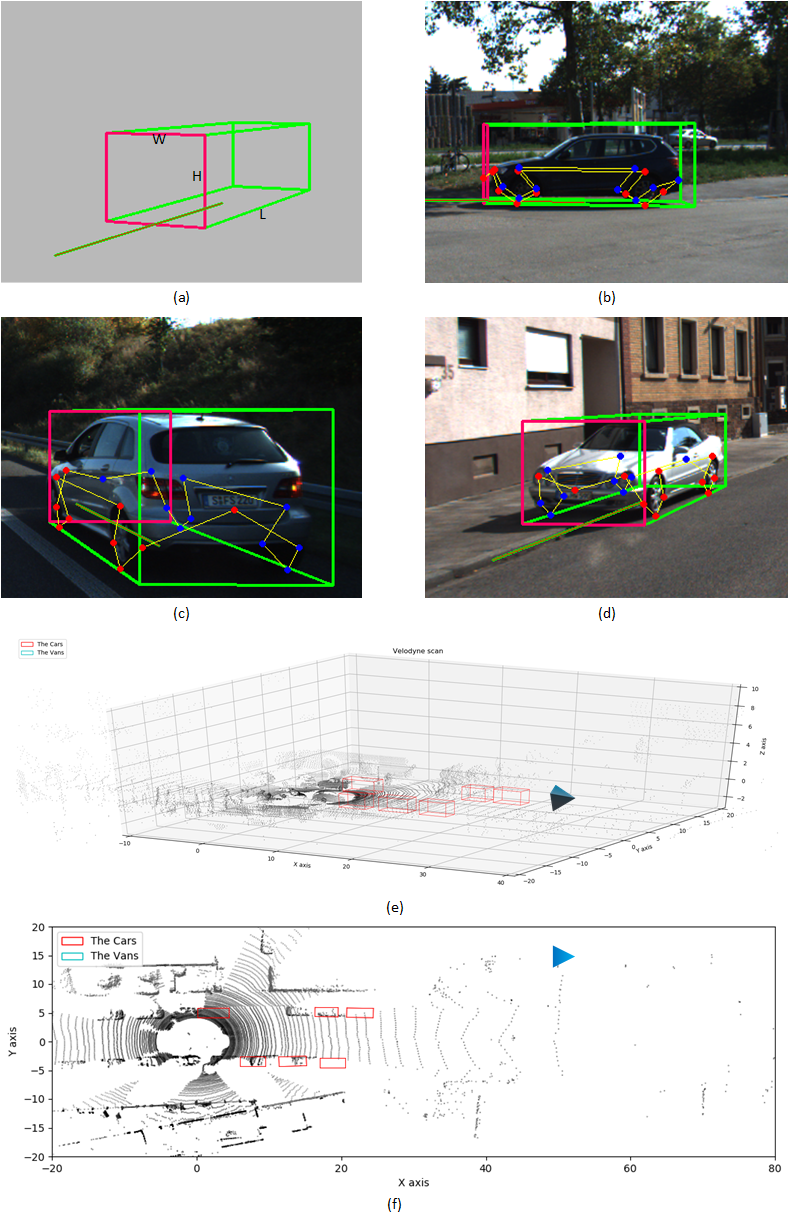
\includegraphics[width=1\textwidth]{visualization.png}
	\caption{Visualization of 3D bounding box and visibility. (a). visualization mechanism, (b). side view of visualization, (c). back view of visualization, (d). front view of visualization}
	\centering
	\label{figure:visualization}
\end{figure}





